
\documentclass[conference]{IEEEtran}

\normalsize

\usepackage{amsmath,amssymb,amsfonts}
\usepackage{textcomp}
\usepackage{xcolor}
\usepackage{booktabs}
\usepackage{colortbl}

% *** CITATION PACKAGES ***
%
\usepackage{cite}
% cite.sty was written by Donald Arseneau
% V1.6 and later of IEEEtran pre-defines the format of the cite.sty package
% \cite{} output to follow that of IEEE. Loading the cite package will
% result in citation numbers being automatically sorted and properly
% "compressed/ranged". e.g., [1], [9], [2], [7], [5], [6] without using
% cite.sty will become [1], [2], [5]--[7], [9] using cite.sty. cite.sty's
% \cite will automatically add leading space, if needed. Use cite.sty's
% noadjust option (cite.sty V3.8 and later) if you want to turn this off.
% cite.sty is already installed on most LaTeX systems. Be sure and use
% version 4.0 (2003-05-27) and later if using hyperref.sty. cite.sty does
% not currently provide for hyperlinked citations.
% The latest version can be obtained at:
% http://www.ctan.org/tex-archive/macros/latex/contrib/cite/
% The documentation is contained in the cite.sty file itself.






% *** GRAPHICS RELATED PACKAGES ***
%
\ifCLASSINFOpdf
   \usepackage[pdftex]{graphicx}
  % declare the path(s) where your graphic files are
  % \graphicspath{{../pdf/}{../jpeg/}}
  % and their extensions so you won't have to specify these with
  % every instance of \includegraphics
  % \DeclareGraphicsExtensions{.pdf,.jpeg,.png}
\else
  % or other class option (dvipsone, dvipdf, if not using dvips). graphicx
  % will default to the driver specified in the system graphics.cfg if no
  % driver is specified.
   \usepackage[dvips]{graphicx}
  % declare the path(s) where your graphic files are
  % \graphicspath{{../eps/}}
  % and their extensions so you won't have to specify these with
  % every instance of \includegraphics
  % \DeclareGraphicsExtensions{.eps}
\fi

% graphicx was written by David Carlisle and Sebastian Rahtz. It is
% required if you want graphics, photos, etc. graphicx.sty is already
% installed on most LaTeX systems. The latest version and documentation can
% be obtained at:
% http://www.ctan.org/tex-archive/macros/latex/required/graphics/
% Another good source of documentation is "Using Imported Graphics in
% LaTeX2e" by Keith Reckdahl which can be found as epslatex.ps or
% epslatex.pdf at: http://www.ctan.org/tex-archive/info/
%
% latex, and pdflatex in dvi mode, support graphics in encapsulated
% postscript (.eps) format. pdflatex in pdf mode supports graphics
% in .pdf, .jpeg, .png and .mps (metapost) formats. Users should ensure
% that all non-photo figures use a vector format (.eps, .pdf, .mps) and
% not a bitmapped formats (.jpeg, .png). IEEE frowns on bitmapped formats
% which can result in "jaggedy"/blurry rendering of lines and letters as
% well as large increases in file sizes.
%
% You can find documentation about the pdfTeX application at:
% http://www.tug.org/applications/pdftex





% *** MATH PACKAGES ***
%
%\usepackage[cmex10]{amsmath}
% A popular package from the American Mathematical Society that provides
% many useful and powerful commands for dealing with mathematics. If using
% it, be sure to load this package with the cmex10 option to ensure that
% only type 1 fonts will utilized at all point sizes. Without this option,
% it is possible that some math symbols, particularly those within
% footnotes, will be rendered in bitmap form which will result in a
% document that can not be IEEE Xplore compliant!
%
% Also, note that the amsmath package sets \interdisplaylinepenalty to 10000
% thus preventing page breaks from occurring within multiline equations. Use:
%\interdisplaylinepenalty=2500
% after loading amsmath to restore such page breaks as IEEEtran.cls normally
% does. amsmath.sty is already installed on most LaTeX systems. The latest
% version and documentation can be obtained at:
% http://www.ctan.org/tex-archive/macros/latex/required/amslatex/math/





% *** SPECIALIZED LIST PACKAGES ***
%
\usepackage{algorithmic}
% algorithmic.sty was written by Peter Williams and Rogerio Brito.
% This package provides an algorithmic environment fo describing algorithms.
% You can use the algorithmic environment in-text or within a figure
% environment to provide for a floating algorithm. Do NOT use the algorithm
% floating environment provided by algorithm.sty (by the same authors) or
% algorithm2e.sty (by Christophe Fiorio) as IEEE does not use dedicated
% algorithm float types and packages that provide these will not provide
% correct IEEE style captions. The latest version and documentation of
% algorithmic.sty can be obtained at:
% http://www.ctan.org/tex-archive/macros/latex/contrib/algorithms/
% There is also a support site at:
% http://algorithms.berlios.de/index.html
% Also of interest may be the (relatively newer and more customizable)
% algorithmicx.sty package by Szasz Janos:
% http://www.ctan.org/tex-archive/macros/latex/contrib/algorithmicx/



% *** ALIGNMENT PACKAGES ***
%
%\usepackage{array}
% Frank Mittelbach's and David Carlisle's array.sty patches and improves
% the standard LaTeX2e array and tabular environments to provide better
% appearance and additional user controls. As the default LaTeX2e table
% generation code is lacking to the point of almost being broken with
% respect to the quality of the end results, all users are strongly
% advised to use an enhanced (at the very least that provided by array.sty)
% set of table tools. array.sty is already installed on most systems. The
% latest version and documentation can be obtained at:
% http://www.ctan.org/tex-archive/macros/latex/required/tools/


%\usepackage{mdwmath}
%\usepackage{mdwtab}
% Also highly recommended is Mark Wooding's extremely powerful MDW tools,
% especially mdwmath.sty and mdwtab.sty which are used to format equations
% and tables, respectively. The MDWtools set is already installed on most
% LaTeX systems. The lastest version and documentation is available at:
% http://www.ctan.org/tex-archive/macros/latex/contrib/mdwtools/


% IEEEtran contains the IEEEeqnarray family of commands that can be used to
% generate multiline equations as well as matrices, tables, etc., of high
% quality.


%\usepackage{eqparbox}
% Also of notable interest is Scott Pakin's eqparbox package for creating
% (automatically sized) equal width boxes - aka "natural width parboxes".
% Available at:
% http://www.ctan.org/tex-archive/macros/latex/contrib/eqparbox/





% *** SUBFIGURE PACKAGES ***
%\usepackage[tight,footnotesize]{subfigure}
% subfigure.sty was written by Steven Douglas Cochran. This package makes it
% easy to put subfigures in your figures. e.g., "Figure 1a and 1b". For IEEE
% work, it is a good idea to load it with the tight package option to reduce
% the amount of white space around the subfigures. subfigure.sty is already
% installed on most LaTeX systems. The latest version and documentation can
% be obtained at:
% http://www.ctan.org/tex-archive/obsolete/macros/latex/contrib/subfigure/
% subfigure.sty has been superceeded by subfig.sty.



%\usepackage[caption=false]{caption}
%\usepackage[font=footnotesize]{subfig}
% subfig.sty, also written by Steven Douglas Cochran, is the modern
% replacement for subfigure.sty. However, subfig.sty requires and
% automatically loads Axel Sommerfeldt's caption.sty which will override
% IEEEtran.cls handling of captions and this will result in nonIEEE style
% figure/table captions. To prevent this problem, be sure and preload
% caption.sty with its "caption=false" package option. This is will preserve
% IEEEtran.cls handing of captions. Version 1.3 (2005/06/28) and later
% (recommended due to many improvements over 1.2) of subfig.sty supports
% the caption=false option directly:
\usepackage[caption=false,font=footnotesize]{subfig}
%
% The latest version and documentation can be obtained at:
% http://www.ctan.org/tex-archive/macros/latex/contrib/subfig/
% The latest version and documentation of caption.sty can be obtained at:
% http://www.ctan.org/tex-archive/macros/latex/contrib/caption/




% *** FLOAT PACKAGES ***
%
%\usepackage{fixltx2e}
% fixltx2e, the successor to the earlier fix2col.sty, was written by
% Frank Mittelbach and David Carlisle. This package corrects a few problems
% in the LaTeX2e kernel, the most notable of which is that in current
% LaTeX2e releases, the ordering of single and double column floats is not
% guaranteed to be preserved. Thus, an unpatched LaTeX2e can allow a
% single column figure to be placed prior to an earlier double column
% figure. The latest version and documentation can be found at:
% http://www.ctan.org/tex-archive/macros/latex/base/



%\usepackage{stfloats}
% stfloats.sty was written by Sigitas Tolusis. This package gives LaTeX2e
% the ability to do double column floats at the bottom of the page as well
% as the top. (e.g., "\begin{figure*}[!b]" is not normally possible in
% LaTeX2e). It also provides a command:
%\fnbelowfloat
% to enable the placement of footnotes below bottom floats (the standard
% LaTeX2e kernel puts them above bottom floats). This is an invasive package
% which rewrites many portions of the LaTeX2e float routines. It may not work
% with other packages that modify the LaTeX2e float routines. The latest
% version and documentation can be obtained at:
% http://www.ctan.org/tex-archive/macros/latex/contrib/sttools/
% Documentation is contained in the stfloats.sty comments as well as in the
% presfull.pdf file. Do not use the stfloats baselinefloat ability as IEEE
% does not allow \baselineskip to stretch. Authors submitting work to the
% IEEE should note that IEEE rarely uses double column equations and
% that authors should try to avoid such use. Do not be tempted to use the
% cuted.sty or midfloat.sty packages (also by Sigitas Tolusis) as IEEE does
% not format its papers in such ways.


%\ifCLASSOPTIONcaptionsoff
%  \usepackage[nomarkers]{endfloat}
% \let\MYoriglatexcaption\caption
% \renewcommand{\caption}[2][\relax]{\MYoriglatexcaption[#2]{#2}}
%\fi
% endfloat.sty was written by James Darrell McCauley and Jeff Goldberg.
% This package may be useful when used in conjunction with IEEEtran.cls'
% captionsoff option. Some IEEE journals/societies require that submissions
% have lists of figures/tables at the end of the paper and that
% figures/tables without any captions are placed on a page by themselves at
% the end of the document. If needed, the draftcls IEEEtran class option or
% \CLASSINPUTbaselinestretch interface can be used to increase the line
% spacing as well. Be sure and use the nomarkers option of endfloat to
% prevent endfloat from "marking" where the figures would have been placed
% in the text. The two hack lines of code above are a slight modification of
% that suggested by in the endfloat docs (section 8.3.1) to ensure that
% the full captions always appear in the list of figures/tables - even if
% the user used the short optional argument of \caption[]{}.
% IEEE papers do not typically make use of \caption[]'s optional argument,
% so this should not be an issue. A similar trick can be used to disable
% captions of packages such as subfig.sty that lack options to turn off
% the subcaptions:
% For subfig.sty:
% \let\MYorigsubfloat\subfloat
% \renewcommand{\subfloat}[2][\relax]{\MYorigsubfloat[]{#2}}
% For subfigure.sty:
% \let\MYorigsubfigure\subfigure
% \renewcommand{\subfigure}[2][\relax]{\MYorigsubfigure[]{#2}}
% However, the above trick will not work if both optional arguments of
% the \subfloat/subfig command are used. Furthermore, there needs to be a
% description of each subfigure *somewhere* and endfloat does not add
% subfigure captions to its list of figures. Thus, the best approach is to
% avoid the use of subfigure captions (many IEEE journals avoid them anyway)
% and instead reference/explain all the subfigures within the main caption.
% The latest version of endfloat.sty and its documentation can obtained at:
% http://www.ctan.org/tex-archive/macros/latex/contrib/endfloat/
%
% The IEEEtran \ifCLASSOPTIONcaptionsoff conditional can also be used
% later in the document, say, to conditionally put the References on a
% page by themselves.





% *** PDF, URL AND HYPERLINK PACKAGES ***
%
%\usepackage{url}
% url.sty was written by Donald Arseneau. It provides better support for
% handling and breaking URLs. url.sty is already installed on most LaTeX
% systems. The latest version can be obtained at:
% http://www.ctan.org/tex-archive/macros/latex/contrib/misc/
% Read the url.sty source comments for usage information. Basically,
% \url{my_url_here}.





% *** Do not adjust lengths that control margins, column widths, etc. ***
% *** Do not use packages that alter fonts (such as pslatex).         ***
% There should be no need to do such things with IEEEtran.cls V1.6 and later.
% (Unless specifically asked to do so by the journal or conference you plan
% to submit to, of course. )


% correct bad hyphenation here
\hyphenation{op-tical net-works semi-conduc-tor}


\begin{document}
%
% paper title
% can use linebreaks \\ within to get better formatting as desired
\title{A Trust-Based Adaptive Authentication Scheme for Space-Air-Ground Integrated NOMA System}
\author{\IEEEauthorblockN{Mingxuan He\IEEEauthorrefmark{1}, Tingyu Cui\IEEEauthorrefmark{1}, Junyu Xiong\IEEEauthorrefmark{1}, Shangwei Zhang\IEEEauthorrefmark{1}\IEEEauthorrefmark{2}, and Huixiang Zhang\IEEEauthorrefmark{1}}

\IEEEauthorblockA{\IEEEauthorrefmark{1}School of Cybersecurity, Northwestern Polytechnical University,
Xi'an, Shaanxi, 710072, China}


\IEEEauthorblockA{\IEEEauthorrefmark{2}E-mail: swzhang@nwpu.edu.cn}}

%Mode Selection of Downlink Coexistent HTC/MTC in D2D-Enabled NOMA Cellular Networks
%Throughput optimization algorithm of maximum likelihood estimation based on Received Signal Strength
%Multi-Agent DRL for Massive Access Coexistent HTC/MTC in D2D-Enhanced Ultra-Dense NOMA System

%A NOMA-Based Multi-Agent Q-Learning Random Access method for MTC in UDNs. Coverage optimization of Downlink NOMA/D2D-Based Coexistent HTC/MTC in Ultra-Dense Networks via Multi-Agent Q-Learning.
%Joint User Pairing and Access Mode Selection of Downlink Coexistent HTC/MTC in NOMA-based D2D communications.


% author names and affiliations
% use a multiple column layout for up to three different
% affiliations


%\author{\IEEEauthorblockN{Shangwei Zhang}
%\IEEEauthorblockA{School of Computer Science and\\Technology\\
%Xidian University\\
%xi'an, Shaanxi 710071\\
%Email: swzhang@mail.xidian.edu.cn}
%\and
%\IEEEauthorblockN{Jiajia Liu}
%\IEEEauthorblockA{School of Computer Science and\\Technology\\
%Xidian University\\
%xi'an, Shaanxi 710071\\
%Email: jjliu@mail.xidian.edu.cn}\\
%
%\and
%\IEEEauthorblockN{James Kirk\\ and Montgomery Scott}
%\IEEEauthorblockA{Starfleet Academy\\
%San Francisco, California 96678-2391\\
%Telephone: (800) 555--1212\\
%Fax: (888) 555--1212}}


%\author{
%\IEEEauthorblockN{Xiao Wang\IEEEauthorrefmark{1}\IEEEauthorrefmark{4},
%Shangwei Zhang\IEEEauthorrefmark{1},
%Jiajia Liu\IEEEauthorrefmark{2} and
%Xinjie Huang\IEEEauthorrefmark{3}}
%\IEEEauthorblockA{\IEEEauthorrefmark{1}School of Computer Science and Technology, Xidian University, China}
%\IEEEauthorblockA{\IEEEauthorrefmark{2}Graduate School of Information Sciences, Tohoku University, Japan}
%\IEEEauthorblockA{\IEEEauthorrefmark{3}NTT Corporation, Japan}
%\IEEEauthorblockA{\IEEEauthorrefmark{4}Email: swzhang@mail.xidian.edu.cn}}% use for special paper notices
%%\IEEEspecialpapernotice{(Invited Paper)}

% make the title area
\maketitle


\begin{abstract}
  The emerging cooperative non-orthogonal multiple access (C-NOMA) technique is expected to be integrated in future space-air-ground integrated networks (SAGIN) to improve network capacity and achieve global coverage. However, the limited resource, untrust NOMA relays and openness channels of SAGIN would inevitably encounter severe data security and privacy violation problems. Many secure access authentication schemes have been developed for SAGIN either by employing physical layer authentication methods for NOMA communication or by utilizing post quantum cryptographic mechanism for orthogonal multiple access networks. In this regard, we propose an adaptive access authentication scheme by considering both trust and untrust NOMA relays to resist quantum attack for C-NOMA communication in SAGIN based on the Number Theory Research Unit scheme. Our scheme can achieve high performance in terms of communication latency and network capacity while guarantee communication security for SAGIN NOMA systems.
\end{abstract}

\begin{IEEEkeywords}
space-air-ground, non-orthogonal multiple access, access authentication
\end{IEEEkeywords}

\section{Introduction}
To fulfill the requirements of huge traffic and seamless connection in the coming Internet of Everything (IoE) era, future sixth generation (6G) wireless communication systems will integrate space, air and ground networks to achieve global coverage \cite{Wang2023}. Besides, emerging non-orthogonal multiple access (NOMA) is expected to further improve the radio access network coverage and spectrum efficiency in future space-air-ground integrated networks (SAGIN) \cite{Wang_TVT2024}. By merging the cooperative communication and NOMA techniques, cooperative NOMA (C-NOMA) was proposed in literature \cite{Ding_CL2015} to enhance the NOMA communication by employing the near user as a relay in each NOMA group. Such a working way can obtain a higher performance gains than traditional NOMA in network capacity. Accordingly, the C-NOMA technique is supposed to be incorporated into SAGIN to achieve massive connectivity and higher spectrum efficiency for various potential IoE applications \cite{Qin_TWC2024}. Although the utilization of NOMA technique holds great promise for future SAGIN, it will inevitably bring security issues like privacy information leakage, forgery attack, etc. One important fact is that the receiver in a typical NOMA group can decode the strongest signal of other user. Moreover, the NOMA group is generally determined based on channel quality rather than on security concerns. As such, confidential or sensitive data might be transmitted through insecure relays in each C-NOMA group.

To tackle this problem, one feasible direction is to explore advanced access authentication scheme, which is primarily design for orthogonal multiple access (OMA) communication systems. For space and ground integrated networks, Chen \textit{et al} in \cite{Chen_ICNP2023} investigated an authentication scheme by utilizing a wireless security negotiation protection process. For NOMA communication systems, recent research works commonly focus on the physical layer authentication scheme. The authors in \cite{Zhang2021} proposed a group authentication mechanism by taking the advantages of NOMA and the irreversibility of hash operation for massive machine type communication systems. Considering the security problem caused by users colluding with the adversary, Xie \textit{et al} in \cite{Xie2020} proposed three physical layer authentication schemes with shared authentication tag, superimposed independent authentication tags and time division multiplexing authentication tags for NOMA systems. Based on this work, they further developed a privacy-preserving authentication scheme to improve the system authentication performance \cite{Xie_JSAC2022}.

The above schemes have not paid attention to the secure access authentication against quantum attack, especially in SAGIN. Accordingly, researchers have tended to improve the access authentication scheme based on the post quantum cryptographic mechanism. For instance, the authors in \cite{Wang_GLOBECOM2022} designed a lattice based anonymous access authentication scheme by utilizing the Number Theory Research Unit (NTRU) scheme into the key generation process. While Wang \textit{et al} developed a NTRU based mutual authentication mechanism with the key generated based on a hash chain \cite{Wang_TITS2024}. Note that the access authentication schemes to resist the quantum attacks are mostly designed for OMA communication systems. Therefore, how to design efficient schemes to take the merits of both C-NOMA and post quantum cryptographic mechanism in future SAGIN is still an open problem. In light of the above considerations, we in this paper investigate a NTRU based authentication scheme for C-NOMA communications in SAGIN. Our goal is to achieve secure communication with guaranteed performance by flexibly implementing security configuration within each C-NOMA group. Specifically, we design an adaptive authentication scheme for SAGIN C-NOMA communication by considering both trust and untrust relays. Besides, we also employ a Certification Authority (CA) and digital certificate technology to ensure the security of the NTRU public key.
\section{System Models} \label{section:model}
As illustrated in Fig. \ref{fig_system_model}, we consider a typical SAGIN downlink power-domain NOMA network systems containing satellites, unmanned aerial vehicles (UAV) and ground users. For sake of network capacity and spectrum efficiency, we assume both UAVs and ground users tend to connect to the satellite for data transmission via NOMA communication. If receivers in the same NOMA group can connect to each other, then C-NOMA communication will be constructed by establishing direct wireless links between them, so as to improve the data transmission capacity as much as possible. For ease of analysis, we consider the scenarios with each NOMA group having two users. Thereby, the tansmit power is divided into two parts, which are devoted to the near and far users in each NOMA group, respectively. It is worth noted that UAVs in the air commonly have much better channel quality (i.e., mostly line-of-sight channel) and higher computational capabilities than those of the ground users (i.e., probably non line-of-sight channel and IoT devices), so they might perform successive interference cancelation (SIC) if employ NOMA technique. Hence, we assume UAVs in the SAGIN can be employed as a relay in each C-NOMA group. For the public key authentication, we assume the public key for space , air and ground communication devices relies on a trusted Certification Authority (CA). The CA provides digital certificates for each devices, verifies the legitimacy of their identities, and facilitates the exchange of public keys.

%In terms of access authentication modes, the satellite delivers data to ground terminals through cooperative multi-hop transmission, utilizing a hybrid Orthogonal Multiple Access (OMA) and Non-Orthogonal Multiple Access (NOMA) scheme for multi-user access. The LEO satellite communicates with ground infrastructure and UAVs via OMA links, transmitting data from the data network to devices closer to the ground. UAVs can communicate directly with the satellite or form a NOMA group with ground terminals, marked by the white area. Acting as relays between the satellite and ground terminals, UAVs help extend the satellite's signal coverage.The ground terminals, located at the lowest level of the system, include devices such as mobile phones, which are situated within NOMA groups and communicate with UAVs via NOMA links. Within the NOMA groups, users utilize NOMA technology to share the same resources, enabling simultaneous signal transmission through resource multiplexing.

For sake of threat model, we in this paper consider the Dolev-Yao model which is a commonly used framework for analyzing security protocols, assuming that attackers have full control over network communications with the capabilities to intercept, modify, forge, and replay messages. Specifically, this model defines the attacker’s abilities as follows:
\begin{itemize}
\item[$\bullet$] The attacker can capture all data transmitted over wireless links between UAVs and users.

\item[$\bullet$] The attacker can send arbitrary data over wireless links to any UAV or satellite.

\item[$\bullet$] The attacker is able to obtain certain users’ short-term keys used for secure communication.

\item[$\bullet$] The attacker is unable to break specific cryptographic primitives, such as symmetric encryption and hash functions. That is, the attacker cannot recover plaintext from ciphertext or forge valid message authentication codes without getting the key.

\item[$\bullet$] The attacker is unable to solve the shortest vector problem (SVP) in lattice-based cryptography.
\end{itemize}
\begin{figure}[!t]
\centering
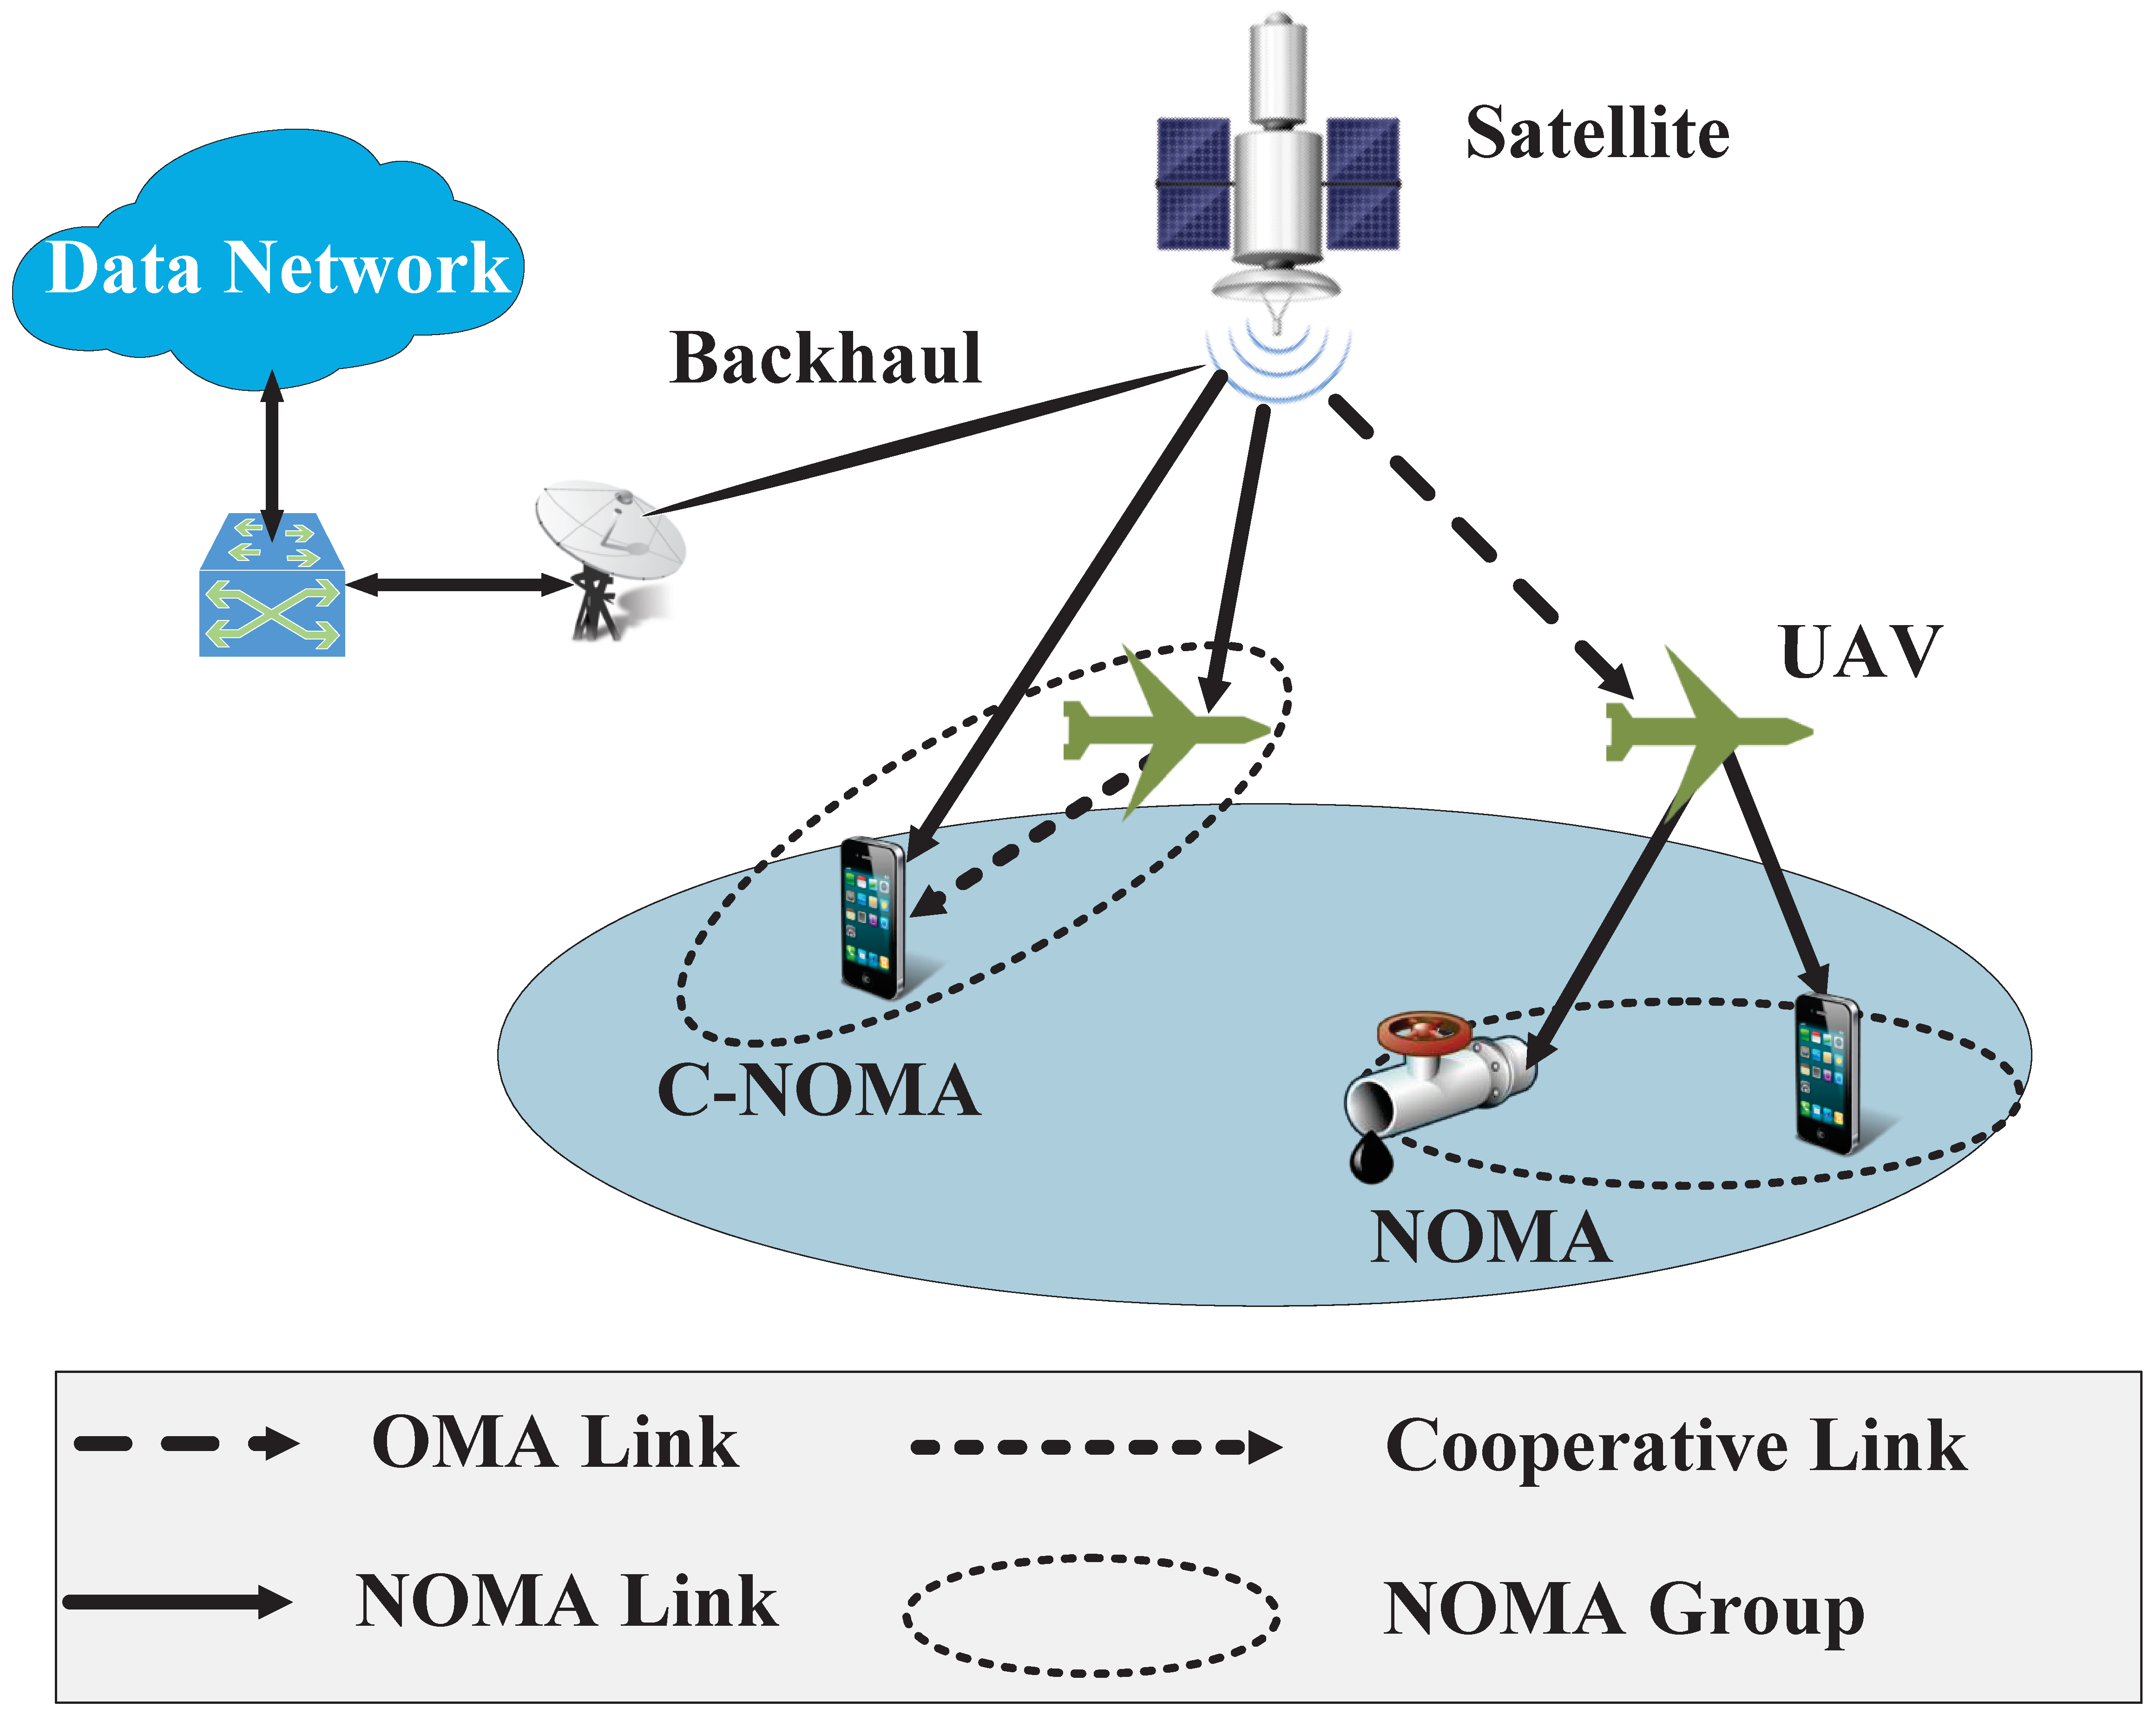
\includegraphics[width=3.0in]{fig_system_model}
\caption{Illustration of space-air-ground integrated NOMA system.}
\label{fig_system_model}
\end{figure}

\section{The Proposed Scheme}
In order to design an authentication scheme to resist quantum attacks while guarantee C-NOMA performance in SAGIN, we first propose a key negotiation mechanism in this part. Below is the symbol table for this authentication scheme.

\begin{table}[!htbp]
\centering
\caption{LIST OF VARIABLES}\label{tab:variable}
%\begin{tabular}{l|l}
\begin{tabular}{>{\columncolor{white}}c | >{\columncolor{white}}c}
\toprule
\hline
\textbf{Variable}& \textbf{Description}\\
\hline
$||$ & Connector \\
\hline
$U_i$ & The $i$th user \\
\hline
$C_i$ & The $i$th ciphertext \\
\hline
$Pub_i$ & The public key of user $i$\\
\hline
$Priv_i$ & The private key of user $i$ \\
\hline
$SK_{i,j}$ & Session key between user $i$ and user $j$ \\
\hline
$SK_{temp_{i,j}}$ &Temporary session key between user $i$ and user $j$ \\
\hline
$MK$ & MAC key \\
\hline
$MAC(key,msg)$ & The message authentication code function \\
\hline
$T$ & Validity time \\
\hline
$DF()$ & Decode-and-Forward message \\
\hline
$rand()$ & The random number generation fuction \\
\hline
$enc(key, data)$ & Encryption of data using key \\
\hline
$dec(key, data)$ & Decryption of data using key \\
\hline
$hash(key, data)$ & Use private key to hash data  \\
\hline
$Cert_i$ & Digital certificates of user $i$\\
\hline
$HKDF()$ & HMAC-based key derivation function \\
\hline
\end{tabular}
\end{table}


\subsection{System Establishment Phase}

%\cite{Wang_GLOBECOM2022}

%NTRU is defined in the polynomial rings $R_q = \mathbb{Z}_q[x]/(x^N - 1)$ , where $N$ is a positive prime,$p$ and $q$ are two integer, $q \gg p,gcd(p,q)=1$. By selecting appropriate random polynomials $f$ and $g$, such that $f \cdot f^{-1}_q \equiv 1 \pmod{q}$ , $f \cdot f^{-1}_p \equiv 1 \pmod{p}$.Let $h = f^{-1} \ast g \pmod{q}$,then the associated NTRU lattice $\Lambda_{h,q}$ is represented as:
%  \[
%    \Lambda_{h,q} = \begin{bmatrix} C(h) & I_n \\ I_n & O_n \end{bmatrix}
%  \]
%where $C(h)$ is the convolution matrix generated by the polynomial $h$,$I_n$ is the $n \times n$ identity matrix,and $O_n$ is the $n \times n$ zero matrix.

%\textbf{Encryption process}:
%
%First, the message $m$ is converted into a polynomial form $m(x)$, represented as a coefficient vector, with $m(x)$ having a degree less than $N-1$.
%
%Next, a polynomial $r(x) \in R_q$ is randomly selected with coefficients following a Gaussian distribution.   The ciphertext $c(x)$ is then generated using the following equation
%
%\[
%  c(x) = p \cdot r(x) \ast h(x) + m(x) \pmod{q}
%\]
%where $\ast$ denotes polynomial convolution. This formula ensures the mixing of the message $m(x)$ with the random polynomial $r(x)$.
%
%\textbf{Decryption process}:
%
%To decrypt the ciphertext $c(x)$ , the private key polynomial $f(x)$ is used as follows:
%\[
% a(x) = f(x) \ast c(x) \pmod{q}
%\]
%
%\[
% m(x) = f^{-1}_p \ast a(x) \pmod{q}
%\]
%Message Recovery: Since $c(x)$ contains a mixture of the message polynomial $m(x)$ and the random polynomial $r(x)$,the process of reducing the modulus $p$ can extract the information of $m(x)$.
%
%The proposed authentication scheme in this article includes the following three entities: the satellite (S), User 1 $(U_1)$, and User 2 $(U_2)$. In this scheme, the satellite acts as the signal transmitter, while $U_1$ and $U_2$ act as receivers, forming a NOMA group.


During the system initialization phase, the satellite, $U_1$ and $U_2$ generate their respective NTRU key pairs. Each user's key pair contains a public key and a private key, which are used for subsequent authentication and communication encryption. We denote the satellite's key pair as $(Pub_S, Priv_S)$, $U_1$'s key pair as $(Pub_{U_1}, Priv_{U_1})$, and $U_2$'s key pair as $(Pub_{U_2}, Priv_{U_2})$.


In the public key exchange process, all users submit their generated public keys (i.e., $Pub_S, Pub_{U_1}, Pub_{U_2}$) to the CA (Certificate Authority) for registration. After verifying the identity of each user, the CA uses its private key to generate digital certificates $Cert_S, Cert_{U_1}, Cert_{U_2}$. Each certificate includes a user identifier (ID), a public key, a validity period and a CA signature. Taking the public key exchange between satellite (SAT) and $U_1$ as an example, the SAT sends its certificate $Cert_S$ to $U_1$. $U_1$ uses the CA's public key to verify the legitimacy of $Cert_S$, then $U_1$ returns its certificate $Cert_{U_1}$ to the satellite. The SAT uses the CA's public key to verify the validity of $Cert_{U_1}$. If the verification is successful, the SAT and $U_1$ can securely share each other’s public keys $Pub_S$ and $Pub_{U_1}$. Similarly, the public key exchange mechanism between the SAT and $U_2$, $U_1$ and $U_2$, can be realized by utilizing the above method.

\begin{figure}[!t]
\centering
\includegraphics[width=3.0in]{fig_relation_illustration}
\caption{Illustration of secure NOMA communication mechanism with trust and untrust relays.}
\label{fig_relation_illustration}
\end{figure}

\begin{figure}[h]
  \centering
  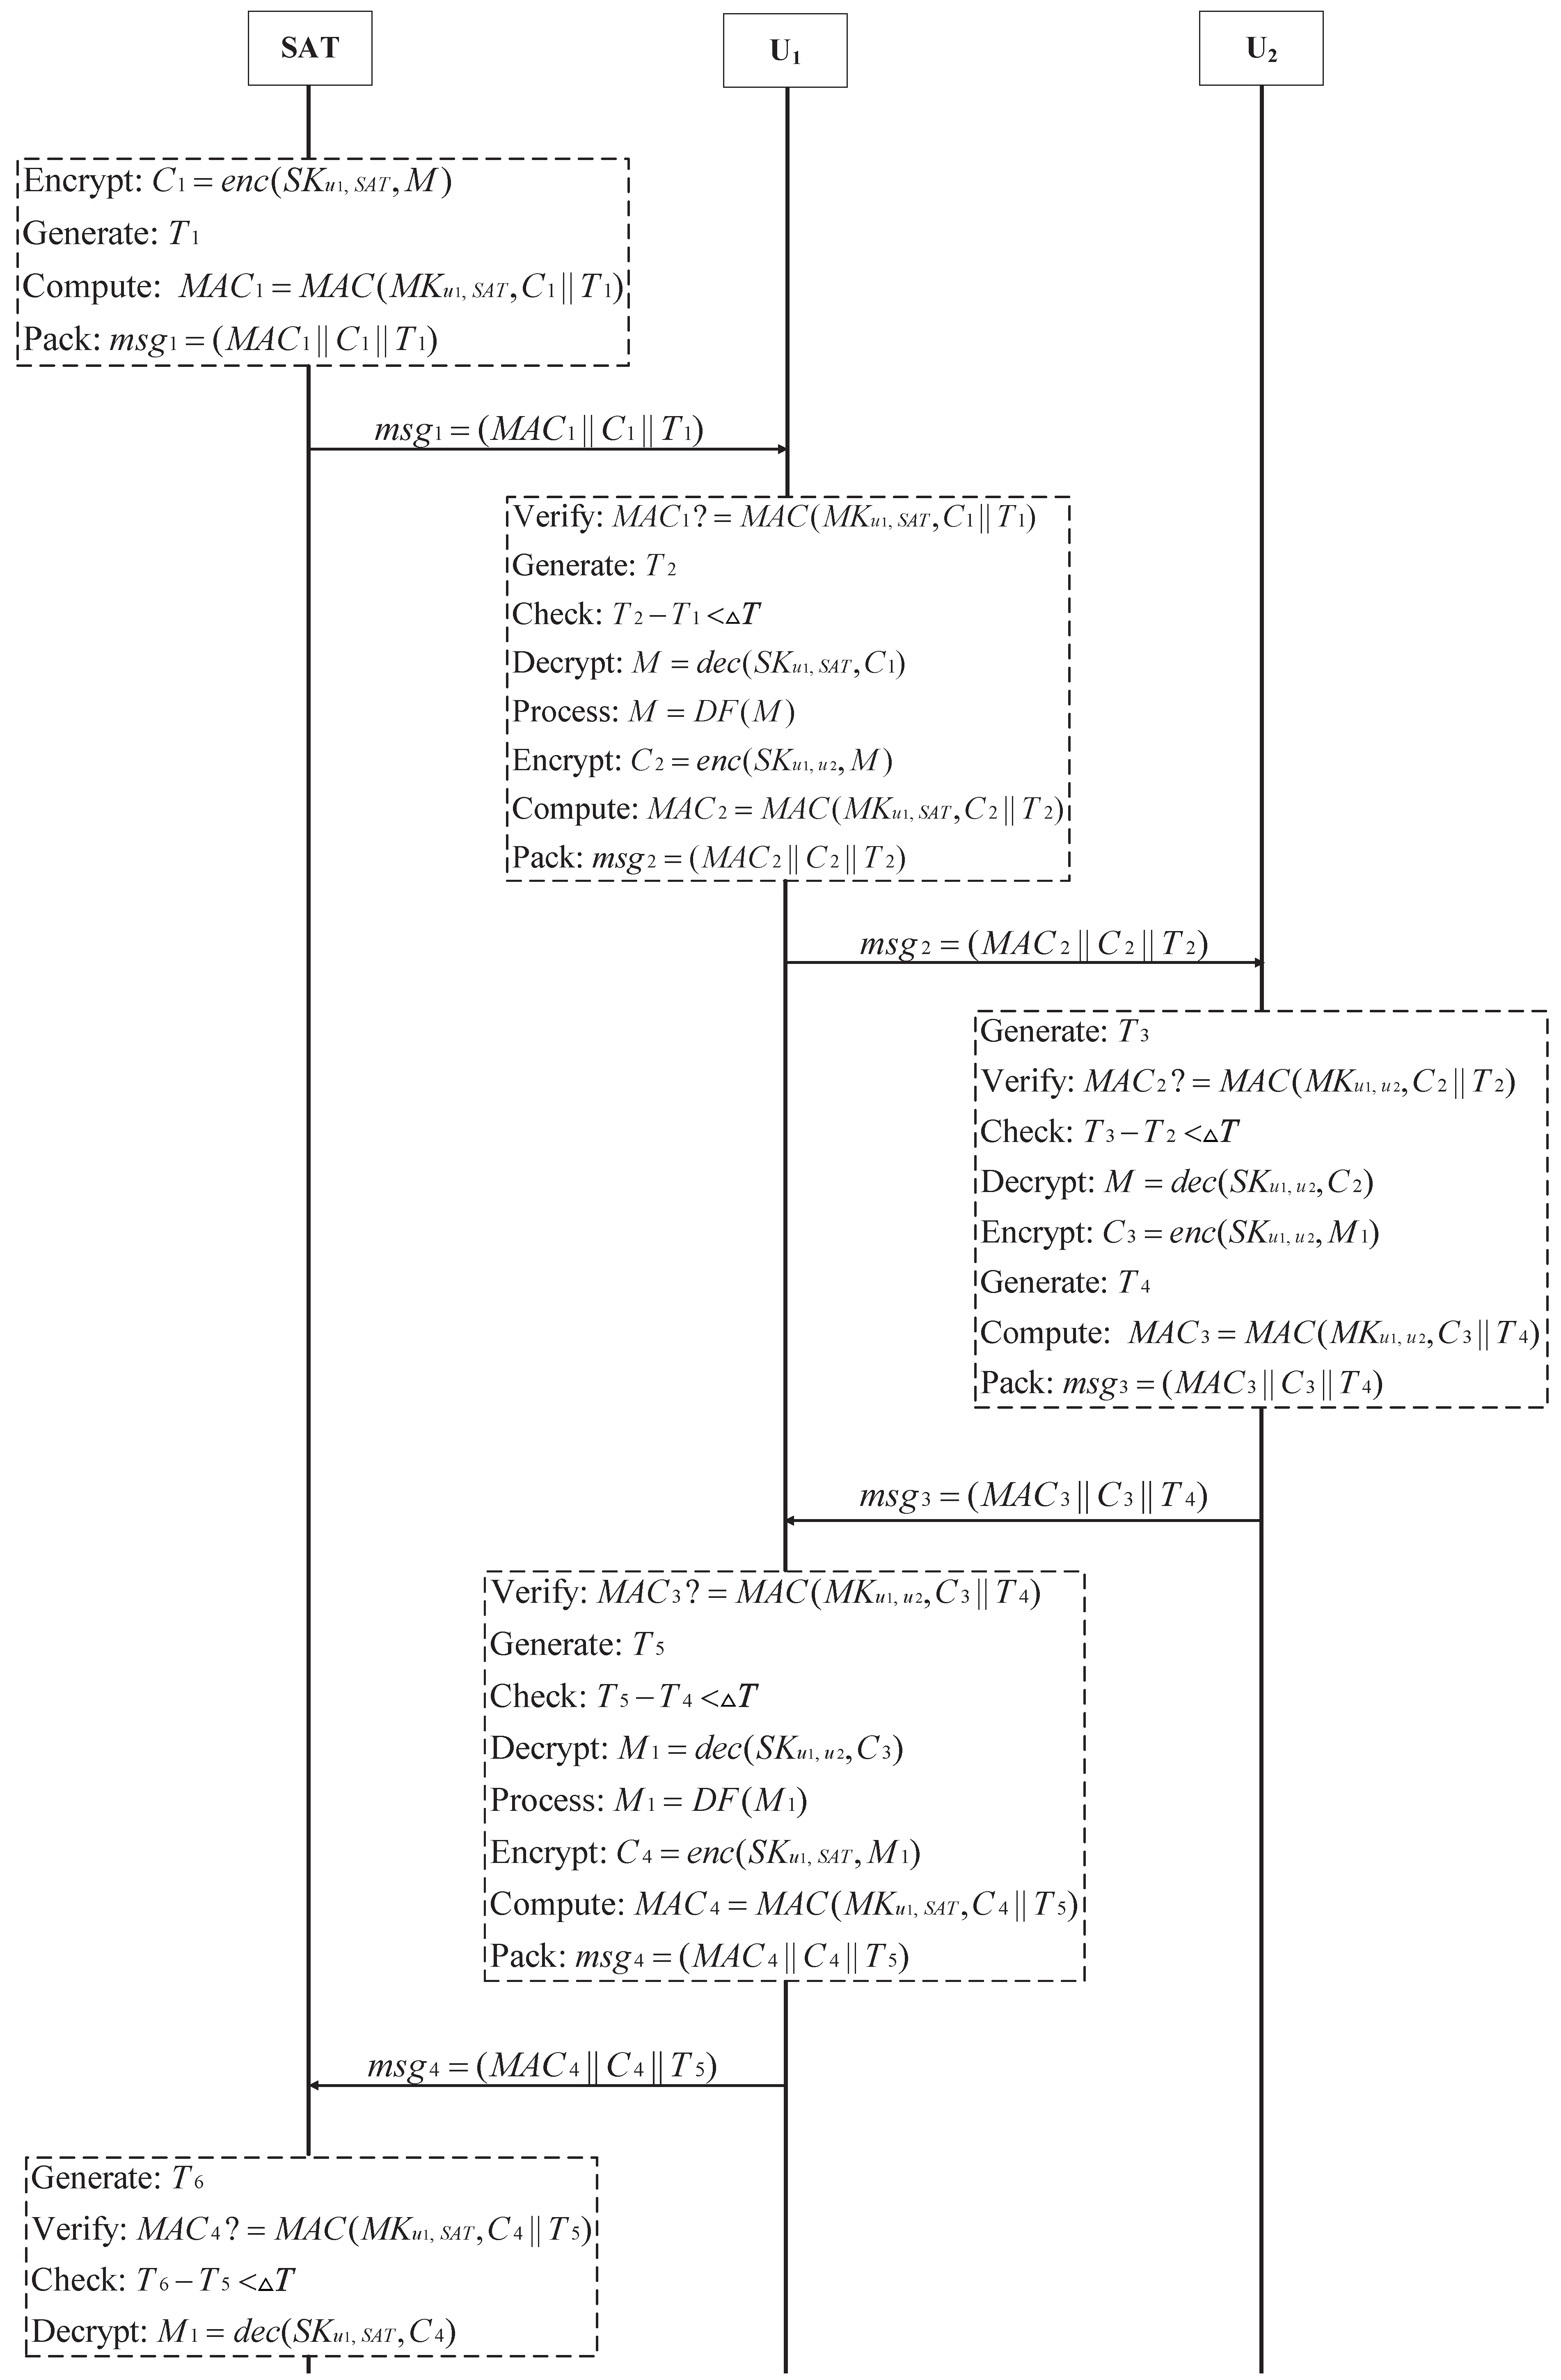
\includegraphics[width=3.5in]{fig_trust_mode}
  \caption{ Interaction diagram of mutual authentication between satellite and NOMA group for trust mode}
  \label{fig_trust_mode}
  \end{figure}

\subsection{Key Negotiation Phase}
In this section, we give the key negotiation process among $U_2$, $U_1$ and SAT. Taking the key negotiation between $U_1$ and $U_2$ as an example, the $U_2$ firstly verifies $U_1$'s certificate and obtains $U_1$'s public key $Pub_1$. Then $U_2$ generates a random number $r_1$ which is further encrypted by using $Pub_1$. After creating the ciphertext $C_1$, $U_2$ generates a validity time $T_1$ and calculates a hash value $H_1 = H(Hello1||C_1||H(r_1)||T_1)$ to ensure data integrity. Finally, $U_2$ sends the message $(Hello1, C_1, Cert_{U_2}, H_1)$ to $U_1$. After receiving the $U_2$'s message, $U_1$ first verifies $U_2$'s certificate $Cert_{U_2}$ and obtains $Pub_2$ if the verification is passed. Then, $U_1$ uses its private key to decrypt the ciphertext $C_1$ to get the random number $r_1'$, which is used to verify the hash value $(H1)'$. $U_1$ also checks the validity of $T_1$. If the verification fails, an error message will be sent to $U_2$ and the negotiation process is terminated. If the verification passes, $U_1$ will generate a random number $r_2$ which is further encrypted by using $Pub_2$ to create the ciphertext $C_2$. Then $U_1$ generates a validity time $T_2$, creates a session key $SK_{U_1,U_2}$ and calculates a hash value $H(r_2)= H(Hello2||C_2||H(r_2)||T_2)$ to ensure data integrity. Finally, $U_1$ sends back $(Hello2, C_2, Cert_{U1}, H_2)$ to $U_2$.

$U_2$ decrypts $C_2$ by using its private key to obtain the random number $r_2'$ after receiving $U_1$'s message. Then $U_2$ verifies the validity of hash value $H_2'$ and $T_2$. If $H_2'$ and $T_2$ are valid, $U_2$ will calculate the session key $SK_{U_2,U_1}$ and generate an integrity hash value $H(All Messages_1)$ for all messages. Later, $U_1$ receives and verifies the hash value $H'(All Messages_1)$ from $U_2$. If $H'(All Messages_1)$ is valid, $U_1$ will send a hash value $H(All Messages_2)$ back to $U_2$. Finally $U_1$ verifies the hash value $H'(All Messages_2)$ from $U_2$. The key negotiation phase between the SAT and $U_2$, SAT and $U_1$, can also be executed by similarly employing the same method.

\subsection{Secure NOMA Communication Process Phase}
We in this part design a secure NOMA communication mechinsm for both trust and untrust relay scenarios. As illustrated in Fig. \ref{fig_relation_illustration}, the satellite establishes a secure communication link between the near user $U_1$ (resp. $U_3$) and the far user U2 (resp. $U_4$), where the  $U_1$ (resp. $U_3$) acts as a relay in the NOMA group. At the beginning of the communication, $U_2$ (resp. $U_4$) can choose to use the trust mode or untrust mode if the corresponding relay is secure or not. In other words, different modes determine whether the relay can get the plaintext data during the relaying process.



Before the communication begins, the satellite, $U_1$, and $U_2$ first generate the MAC key $MK_{i,j}$ based on the session key $SK_{i,j}$ obtained from the previous handshake exchange. The MAC key is calculated as $MK_{i,j} = HKDF(SK_{i,j})$.

1) \textit{\textbf{Trust Mode}}


\quad



(1) $SAT \rightarrow U_1$

Step 1: As illustrate in Fig. \ref{fig_trust_mode}, $U_2$ sends a trust mode communication request to the satellite. Upon receiving the request, the SAT encrypts the plaintext message $M$ using the session key $SK_{U_1,SAT}$ to generate the ciphertext $C_1$ = $enc(SK_{SAT,U_1},M)$.

Step 2: SAT generates the current valid time $T_1$ and calculates $MAC_1 = MAC(MK_{SAT,U_1}, C_1||T_1)$.

Step 3: The satellite packages the message $msg_1=(MAC_1||C_1||T_1)$ and sends $msg_1$ to $U_1$.

(2) $U_1 \rightarrow U_2$

%The purpose of this process is to perform Decode-and-Forward on the message
Step 1: $U_1$ first verifies the MAC value using $MK_{U_1,SAT}$ and verifies the validity of the timestamp $T_1$. If the timestamp is valid and the MAC verification passes, the message will be accepted. Otherwise, the message will be discarded.

Step 2: $U_1$ decrypts the ciphertext $C_1$ using the session key $SK_{U_1,SAT}$ to obtain the original plaintext data $M = dec(SK_{U_1,SAT},C_1)$. Then $U_1$ generates the current valid timestamp $T_2$.

Step 3: $U_1$ encrypts the data $M$ using the session key $SK_{U_1,U_2}$ to generate the new ciphertext $C_2$ = $enc(SK_{U_1,SAT},M)$ .

Step 4: $U_1$ uses the MAC key $MK_{U_1,U_2}$ to generate $MAC_2$, where $MAC_2 = (MK_{U_1,U_2}, C_2||T_2)$.

Step 5: $U_1$ packages the message $msg_2=(MAC_2||C_2||T_2)$ and sends it to $U_2$.

(3) $U_2$ verifies the legitimacy of the message and decrypts it to obtain $M$.

Step 1: $U_2$ verifies the MAC value using $MK_{U_2,U_1}$ and verifies the validity of the timestamp $T_2$. If the timestamp is valid and the MAC verification passes, the message will be accepted. Otherwise, the message will be discarded.

Step 2: $U_2$ uses the session key $SK_{U_2,U_1}$ to decrypt the ciphertext $C_2$ and recover the original plaintext data $M = dec(SK_{U_2,U_1},C_2)$.

At this point, the satellite has successfully transmitted a message to $U_2$ in the downlink. The mechanism for the uplink case is similar to the above steps and we omit it here.



2) \textit{\textbf{Untrust Mode}}

\begin{figure}[htbp]
  \centering
  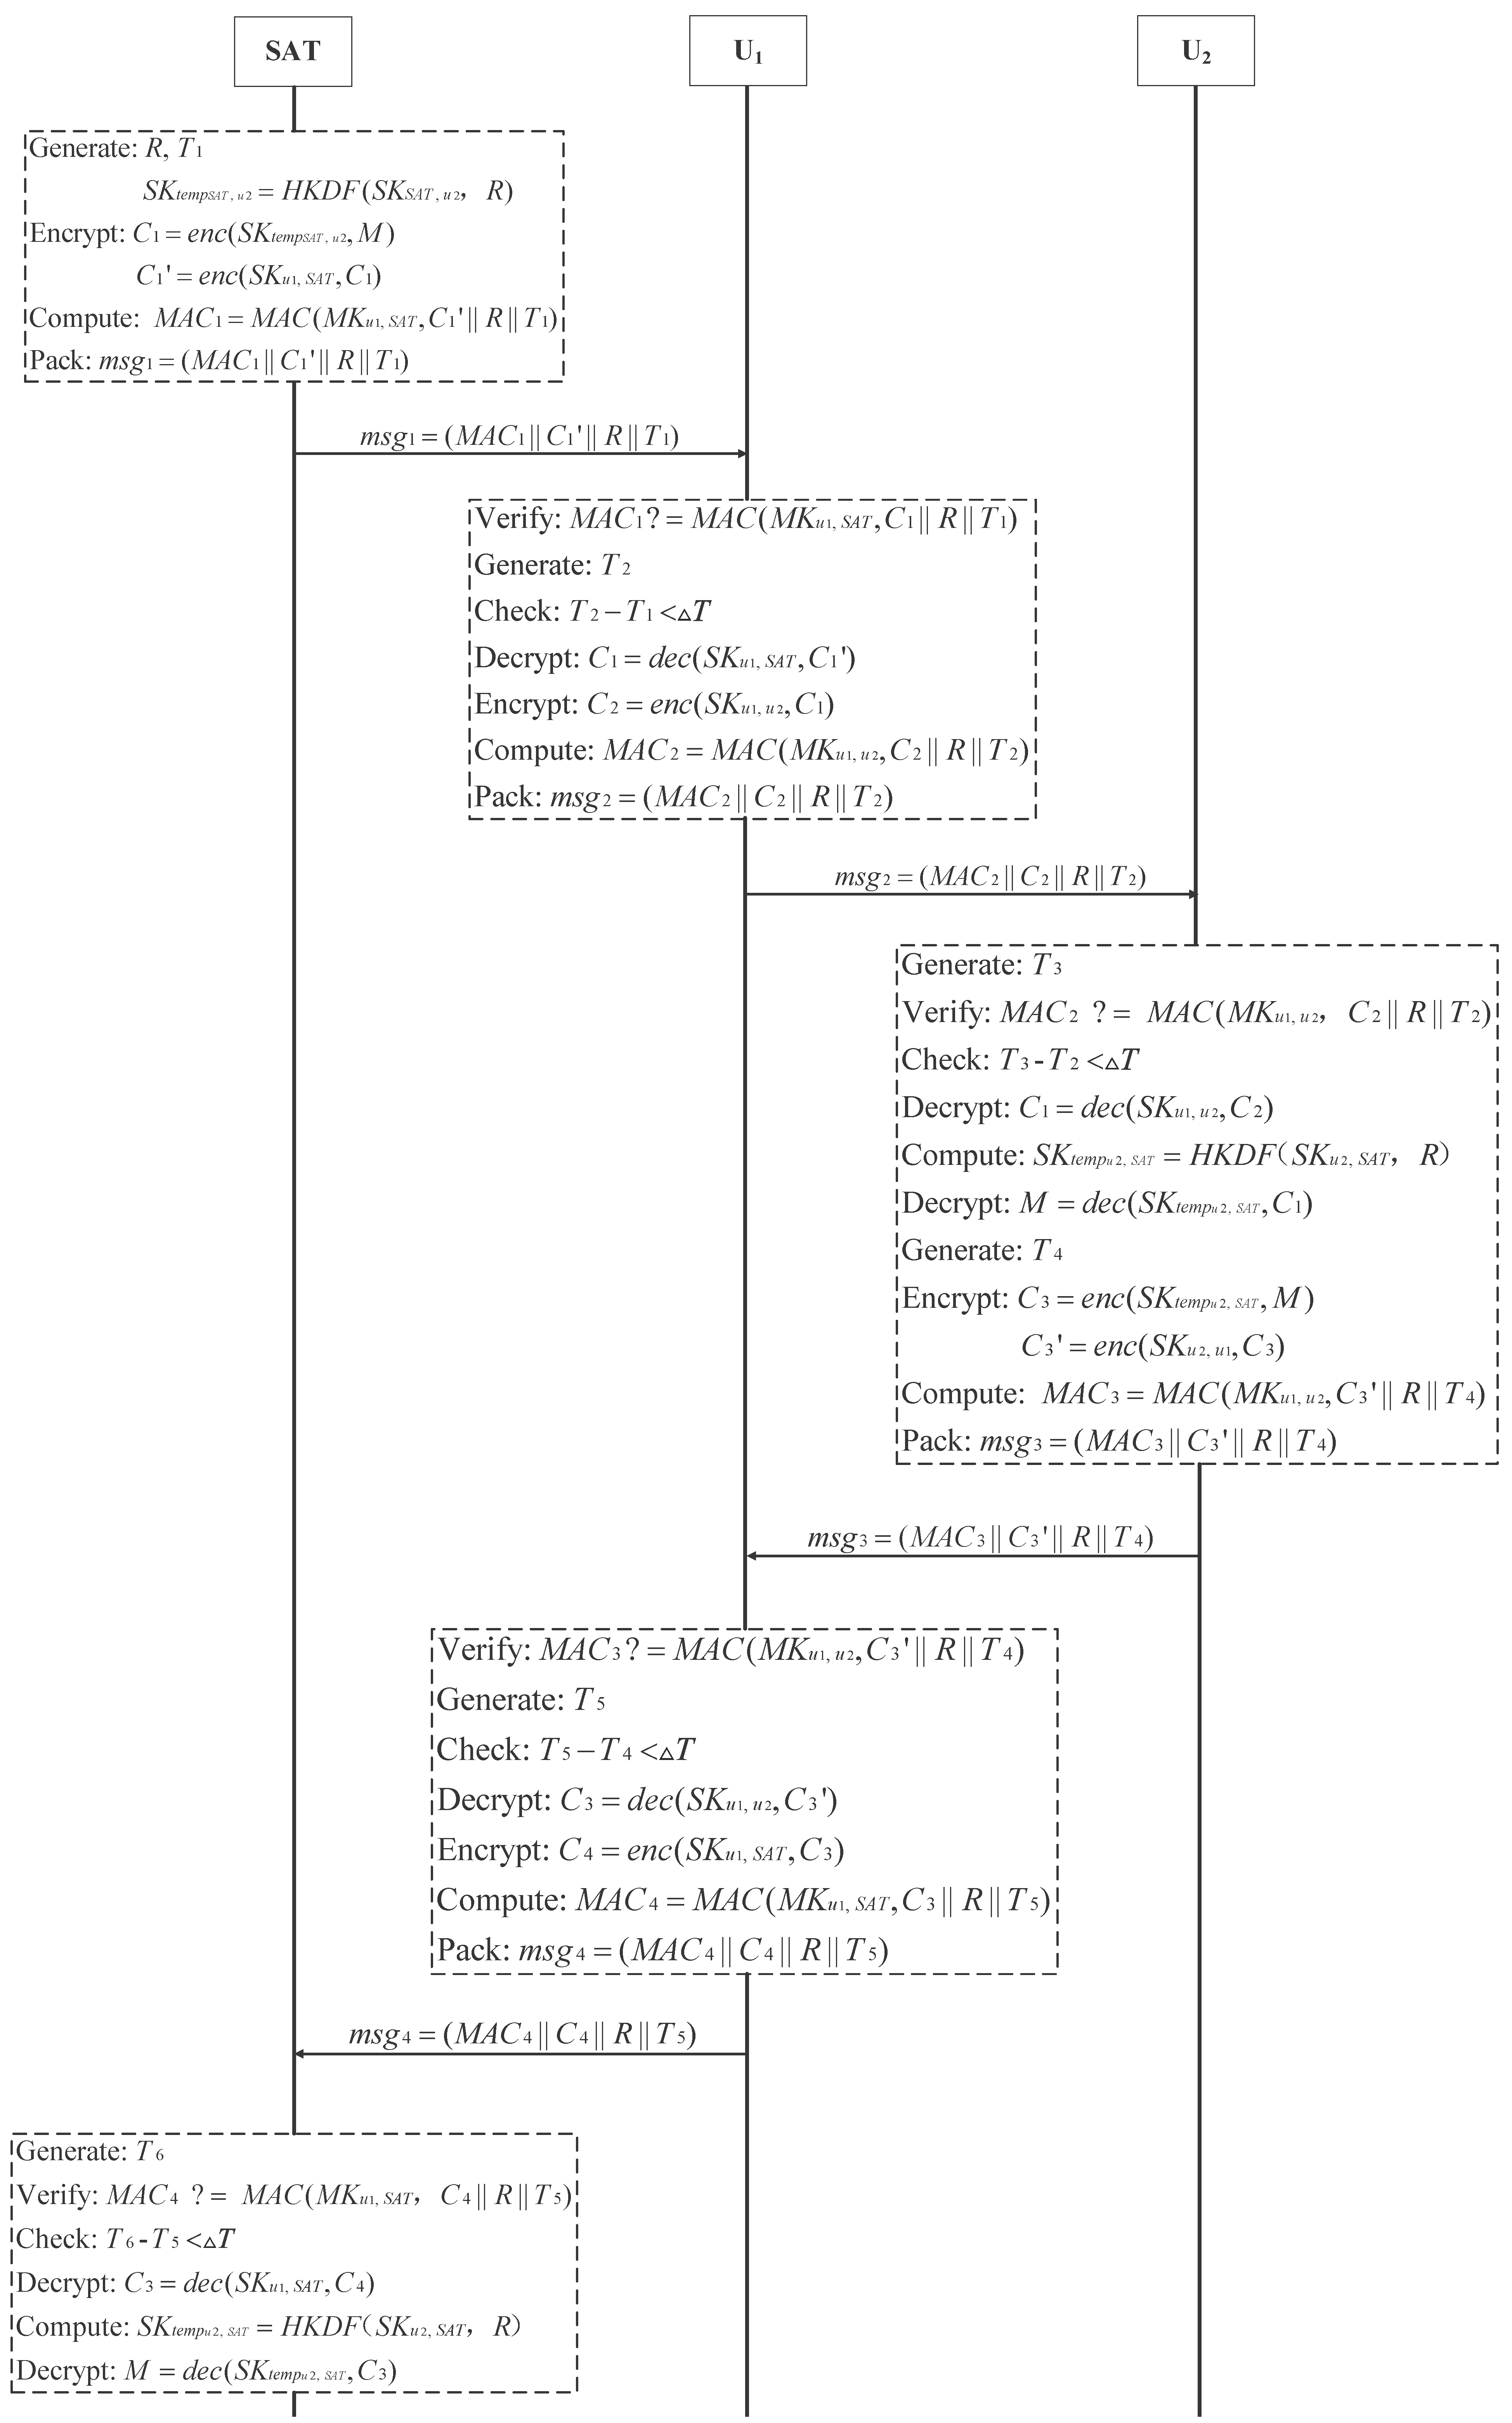
\includegraphics[width=3.5in]{fig_untrust_mode}
  \caption{Interaction diagram of mutual authentication between satellite and NOMA group for untrust mode}
  \label{fig_untrust_mode}
  \end{figure}

(1) $SAT \rightarrow U_1$

Step 1: As illustrate in Fig. \ref{fig_untrust_mode}, the SAT periodically generates a new random number $R = rand()$, which serves as a seed for mixing the temporary session key $SK_{temp_{SAT,U_2}}=HKDF(SK_{SAT,U_2}, R)$. $SK_{temp_{SAT,U_2}}$ is only used for encrypting communication in this session.

Step 2: The satellite encrypts the plaintext message using the temporary session key $SK_{temp_{SAT,U_2}}$ to produce ciphertext $C_1$ = $enc(SK_{temp_{SAT,u_2}},M)$, and subsequently encrypts the ciphertext message $C_1'$ using the key $SK_{U_1,SAT}$ to generate ciphertext $C_1'$ =$enc(SK_{temp_{SAT,U_1}},C_1)$.

Step 3: It then generates the current valid timestamp $T_1$ and calculates the message authentication code as $MAC_1 = MAC(MK_{U_1,SAT}, C_1'||R||T_1)$ using $MK_{SAT,U_1}$. Finally, the satellite packages the message $msg_1=(MAC_1||C_1'||R||T_1)$ and sends it to $U_1$.

(2) $U_1 \rightarrow U_2$

Step 1: $U_1$ first verifies the MAC value using the shared MAC key $MK_{U_1,SAT}$ and verifies the validity of the timestamp $T_1$. If the timestamp is valid and the MAC verification passes, the message will be accepted. Otherwise, the message will be discarded.

Step 2: $U_1$ decrypts the ciphertext $C_1'$ using the session key $SK_{U_1,SAT}$ to obtain the ciphertext $C_1$ = $dec(SK_{U_1,SAT},C_1')$.

Step 3: $U_1$ generates the current valid timestamp $T_2$.

Step 4: $U_1$ encrypts the data using the session key $SK_{U_1,U_2}$ to generate the new ciphertext $C_2$ = $enc(SK_{U_1,U_2},C_1)$ and using the MAC key $MK_{U_1,U_2}$ to generate $MAC_2$, where $MAC_2 = (MK_{U_1,SAT}, C_2||R||T_2)$.

Step 5: $U_1$ packages the message $msg_2=(MAC_2||C_2 ||R||T_2)$ and sends it to $U_2$.



(3) $U_2$ verifies the legitimacy of the message and decrypts it to obtain $M$

Step 1: $U_2$ verifies the MAC value using the shared MAC key $MK_{U_2,U_1}$. If the timestamp is valid and the MAC verification passes, the message will be accepted. Otherwise, the message will be discarded.

Step 2: $U_2$ uses the session key $SK_{U_1,U_2}$ to decrypt the ciphertext $C_2$ and obtains the ciphertext $C_1$= $dec(SK_{U_1,U_2},C_2)$.

Step 3: $U_2$ calculates the temporary session key

$SK_{temp_{U_2,SAT}}=HKDF(SK_{U_2,SAT}, R)$

Step 4: $U_2$ uses $SK_{temp_{U_2,SAT}}$ to decrypt $C_1$ to retrieve the plaintext $M = dec(SK_{temp_{U_2,SAT}},C_1)$.

At this point, the satellite has successfully transmitted a message to $U_2$ in the downlink. The mechanism for the uplink scenario is similar to these steps and will not be elaborated here.




\section{PERFORMANCE EVALUATION AND ANALYSIS}

In this section, we analyze the effectiveness and security of the proposed scheme and demonstrate the performance advantages of our proposed scheme from two perspectives: communication overhead and computational overhead. Additionally, we employ the formal analysis tool, BAN Logic, to verify the correctness of the proposed scheme. All experiments are conducted on a personal computer equipped with an Intel Core i5-13400F CPU running on a Windows 11 operating system. Through analysis, our scheme can achieve secure authentication, key agreement functions, and supports message accessibility for near users in C-NOMA groups. It also ensures the confidentiality of key agreement, guarantees forward secrecy and backward secrecy.

\subsection{Communication Overhead}
For a complete end-to-end transmission, we use the metric STGD (satellite-to-ground transmission delay, around $4.833ms$ per STGD) raised in the literature \cite{Wang_GLOBECOM2022} to measure the size of communication overhead. Table \text{III} is a comparison of the communication overhead of our scheme with other schemes. As shown in table \text{II}, the scheme in reference \cite{Yantao2010} and \cite{Wang_TITS2024} require four STGD, \cite{Zhou_SCN2020} requires six STGD, and \cite{Wang_GLOBECOM2022} requires two STGD. Compared to these schemes, our proposed scheme only requires two STGD, which is equal to the scheme in \cite{Wang_GLOBECOM2022} and less than the others.


\begin{table}[!htbp]
\centering
\caption{Comparison of Communication Overhead}\label{tab:comparison}
%\begin{tabular}{l|l}
\begin{tabular}{>{\columncolor{white}}c | >{\columncolor{white}}c}
\toprule
\hline
\textbf{Scheme}& \textbf{Communication Overhead}\\
\hline
Y. Zhong, \textit{et al} \cite{Yantao2010} & 4STGD \\
\hline
      Y. Wang, \textit{et al} \cite{Wang_TITS2024} & 4STGD \\
\hline
     Y. Zhou, \textit{et al} \cite{Zhou_SCN2020}  &  6STGD \\
\hline
      S. Wang, \textit{et al} \cite{Wang_GLOBECOM2022} & 2STGD \\
\hline
      OURS & 2STGD \\
\hline
\end{tabular}
\end{table}

\subsection{Computation Overhead}

We define the computational cost as the total time spent on various operations in the entire authentication scheme. The time cost of each type of operation is explained as follows: $T_h (0.186ms)$ is the time cost for Hash Operation, $T_r (0.51ms)$ is the time cost for Random Generation, $T_e (5.8ms)$ is the time cost for modular exponent, $T_{NE} (0.15ms)$ is the time cost for NTRU encryption, $T_{ND} (0.16ms)$ is the time cost for NTRU decryption, $T_{NM} (0.026ms)$ is the time cost for NTRU modulus multiplication, and $T_g (73ns)$ is the time cost for random sampling operation.

From Table \text{III}, it can be seen that the computational overheads of the schemes proposed in \cite{Yantao2010}, \cite{Wang_TITS2024}, \cite{Zhou_SCN2020}, and \cite{Wang_GLOBECOM2022} are 23.944ms, 1.664ms, 1.266ms, and 1.427ms, respectively. While our scheme has a computational overhead of 3.838ms. Although the computational overhead of our scheme is higher than the other three schemes except for \cite{Yantao2010}, \cite{Wang_TITS2024} and \cite{Zhou_SCN2020} require at least 2 additional STGD operations compared to our scheme. \cite{Wang_GLOBECOM2022} has the same number of STGD operations as our scheme, but it cannot complete satellite-ground communication when the user’s channel quality is poor. Therefore, our scheme can achieve better performance than the other four schemes.

\begin{table}[!htbp]
\centering
\caption{Comparison of Computation Overhead}\label{tab:comparison1}
%\begin{tabular}{l|l}
\begin{tabular}{>{\columncolor{white}}c | >{\columncolor{white}}c}
\toprule
\hline
\textbf{Scheme}& \textbf{Authentication delay}\\
\hline
Y. Zhong, \textit{et al} \cite{Yantao2010} & $3T_e + 4T_h$ \\
\hline
      Y. Wang, \textit{et al} \cite{Wang_TITS2024} & $8T_h + T_{NE} + T_{NM}$ \\
\hline
       Y. Zhou, \textit{et al} \cite{Zhou_SCN2020} & $5T_h + T_{NE} + T_{ND} + T_{NM}$ \\
\hline
     S. Wang, \textit{et al} \cite{Wang_GLOBECOM2022} & $6T_h + 8T_g + T_{NE} + T_{ND}$ \\
\hline
      OURS & $4T_h+4T_r+T_{NE}+T_{ND}$ \\
\hline
\end{tabular}
\end{table}

\subsection{Security Analysis}

For security analysis and comparison, we employ the related research to analyze the security of our proposed scheme, as shown in Table \text{IV}. Specifically, Reference\cite{Yantao2010} demonstrates that their protocol is ECK-secure under the Computational Diffie-Hellman (CDH) assumption in the random oracle model. Reference\cite{Wang_TITS2024} and Reference\cite{Zhou_SCN2020} use qualitative security analysis and BAN logic to evaluate the security properties of the proposed scheme. Reference\cite{Wang_GLOBECOM2022} uses a mathematical formalization approach to verify the correctness of its designed protocol, ensuring that the protocol meets various security requirements under the expected security model and assumptions. We compare the security and functional features with four other schemes. To defend against \textbf{replay attacks}, our scheme uses timestamp, random numbers, and MAC to ensure each session key is unique, so that replayed messages cannot pass verification. To resist \textbf{DoS attacks}, Our scheme uses MAC and timestamp to authenticate legitimate requests, discarding expired or forged requests to mitigate the impact of DoS attacks. To defend against \textbf{man-in-the-middle attacks}, Our scheme uses public keys issued by the CA for bidirectional identity verification. This ensures the authenticity of the communication. To resist \textbf{quantum attacks}, our scheme adopts the NTRU encryption algorithm, which relies on a lattice-based design that quantum algorithms cannot efficiently break. Our scheme independently generates session keys through the HKDF function. Even if the current session key is compromised, the keys from previous or future sessions are not impacted. This ensures \textbf{forward and backward security}. Finally, our scheme achieves \textbf{message accessibility for weak-channel users}.

\begin{table*}[!htbp]
\centering
\caption{COMPARISON OF SECURITY AND FUNCTIONAL FEATURES}\label{tab:comparison}
%\begin{tabular}{l|l}
\begin{tabular}{>{\columncolor{white}}c | >{\columncolor{white}}c| >{\columncolor{white}}c| >{\columncolor{white}}c| >{\columncolor{white}}c| >{\columncolor{white}}c}
\toprule
\hline
\textbf{Security Features}& Y. Zhong, \textit{et al} \cite{Yantao2010}& Y. Wang, \textit{et al} \cite{Wang_TITS2024}& Y. Zhou, \textit{et al} \cite{Zhou_SCN2020} & S. Wang, \textit{et al} \cite{Wang_GLOBECOM2022}& \textbf{Ours}\\
\hline
Mutual authentication & $\checkmark$ & $\checkmark$ & $\checkmark$ & $\checkmark$ & $\checkmark$ \\
\hline
Key Agreement & $\checkmark$ & $\checkmark$ & $\checkmark$ & $\checkmark$ & $\checkmark$ \\
\hline
Forward Security & $\checkmark$ & $\checkmark$ & $\checkmark$ & $\checkmark$ & $\checkmark$ \\
\hline
Backward Security & $\checkmark$ & $\checkmark$ &$\checkmark$  & $\checkmark$ & $\checkmark$ \\
\hline
Man-in-the-middle Attack & $\checkmark$ & $\checkmark$ & $\checkmark$ & $\checkmark$ & $\checkmark$ \\
\hline
Replay Attack & $\checkmark$ & $\checkmark$ & $\checkmark$  & $\checkmark$ & $\checkmark$ \\
\hline
Security Formal Proof & $\checkmark$ & $\checkmark$ & $\checkmark$ & $\checkmark$ & $\checkmark$ \\
\hline
Resist Quantum Attack & $\times$ & $\times$ & $\checkmark$ & $\checkmark$ & $\checkmark$ \\
\hline
Message accessibility for near users & $\times$ & $\times$ & $\times$ & $\times$ & $\checkmark$ \\
\hline
\end{tabular}
\end{table*}






\subsection{Correctness Proof}

In this section, we use the Ban logic to prove the correctness and security of the scheme, which is based on a set of specific inference rules that abstract information about entities' beliefs, trust relationships, and the freshness of messages exchanged during protocol interactions to derive whether the final protocol can achieve its expected security goals \cite{Burrows1990}. First, we define the symbols used in Ban logic:

\begin{itemize}

\item[$\bullet$] A and B represent the communicating entities, and $X$ represents the message transmitted in the protocol.

\item[$\bullet$] $P |\equiv X$ denotes that entity $P$ believes $X$ to be true, meaning entity $P$ considers $X$ to be a valid assertion.

\item[$\bullet$] $P \lhd  X$ indicates that entity $P$ has received the message containing $X$.

\item[$\bullet$] $P | \sim  X$ means that entity $P$ once send message $X$. 

\item[$\bullet$] $P | \Rightarrow  X$ means that $P$ has jurisdiction over message $X$.

\item[$\bullet$] $ \# (X)$ denotes that $X$ is fresh.

\item[$\bullet$] ${X}_K$ denotes that message $X$ has been encrypted with key $K$.

\item[$\bullet$] $ P \overset{K}\leftrightarrow Q $ means that the $K$ is shared between $P$ and $Q$.

\item[$\bullet$] $ SK_{U_1,U_{2}}$ represents the session key between $U_1$ and $U_2$, which is used for confidential communication between the two parties.

\item[$\bullet$] $H(X)$ represents the hash value of $X$, which is used for data integrity verification."

\end{itemize}

Here are the definitions of inference rules:

\begin{itemize}

\item[$\bullet$] Message implication rule  $\frac{P |\equiv Q \leftrightarrow K \leftrightarrow P,P \lhd  X_K}{P |\equiv Q |\equiv X}$. This rule indicates that if $P$ shares a secret key $K$ with $Q$ and receives a message $X$ encrypted by $K$, then $P$ believes that $Q$ believes $X$ is true.

\item[$\bullet$] Nonce verification rule $ \frac{P |\equiv \#(x),P |\equiv Q| \sim  X}{P |\equiv Q |\equiv X} $. This rule states that if $P$ believes $X$ is fresh, and also believes that $Q$ has sent $X$, then $P$ can trust the authenticity of $X$.

\item[$\bullet$] Jurisdiction rule $ \frac{P |\equiv Q| \Rightarrow   X,P |\equiv Q |\equiv X}{P |\equiv X} $. If $P$ believes that $Q$ has jurisdiction over $X$, and $P$ trust $Q$'s judgment on the authenticity of $X$, then $P$ can trust $X$.

\item[$\bullet$]Belief transmission rule $ \frac{P |\equiv Q |\equiv X,P |\equiv Q| \sim  X}{P |\equiv X} $. If $P$ believes $Q$ and $P$ believes $Q$ controls $X$, then $P$ can consider $X$ to be true.

\end{itemize}

\textbf{Goals}:
Based on the above BAN symbols and logical definitions, our scheme should achieve the following security objectives.

G1: $U_1|\equiv U_1 \overset{SK_{U1,U2}}\longleftrightarrow U_2$

G2: $U_2|\equiv U_1 \overset{SK_{U1,U2}}\longleftrightarrow U_2$

G3: $U_1|\equiv  U_2|\equiv U_1 \overset{SK_{U1,U2}}\longleftrightarrow U_2$

G4: $U_2|\equiv U_1|\equiv U_1 \overset{SK_{U1,U2}}\longleftrightarrow U_2$

\textbf{Messages}: According to the proposed authentication scheme, we transform the scheme into the following form:

Message1: $U_2 \to  U_1$:

$U_1 \lhd \{ T_1||\{r_1\}Pub_{U_1}||Hello1||H\{Hello1||\{r_1\}Pub_{U_1}||T_1\}\}$

Message2: $U_1 \to  U_2$:

$U_2 \lhd \{ T_2||\{r_2\}Pub_{U_2}||Hello2||H\{Hello2||\{r_2\}Pub_{U_2}||T_2\}\}$

Message3: $U_2 \to  U_1$:

$ U_1 \lhd \{H\{\{ T_1||\{r_1\}Pub_{U_1}||Hello1||H\{Hello1||\{r_1\}Pub_{U_1}||\\T_1\}\},\{T_2||{r_2}Pub_{U_2}||Hello2||H\{Hello2||\{r_2\}Pub_{U_2}||T_2\}\}\}\} $

Message4: $U_1 \to  U_2$:

$U_2 \lhd \{H\{\{H\{\{ T1||\{r_1\}Pub_{U_1}||Hello1||H\{Hello1||\{r_1\}\\Pub_{U_1}||T_1\}\},\{T_2||{r_2}Pub_{U_2}||Hello2||H\{Hello2||\{r_2\}Pub_{U_2}\\||T_2\}\}\}\}\}\}$

\textbf{States}: According to the protocol description, the initial state is as follows

A1: $U_1 \lhd \{r_1\}Pub_{U_1}$

A2: $U_1|\equiv \#(r_1)$

A3: $U_1|\equiv \#(T_1)$

A4: $U_1|\equiv U_2|\Rightarrow U_1 \overset{r_1}\longleftrightarrow U_2$

A5: $U_2 \lhd \{r_2\}Pub_{U_2}$

A6: $U_2|\equiv \#(r_2)$

A7: $U_2|\equiv \#(T_2)$

A8: $U_2|\equiv U_1|\Rightarrow U_1 \overset{r_2}\longleftrightarrow U_2$

A9: $U_2|\equiv U_2 \overset{r_1}\longleftrightarrow U_1$

A10: $U_1|\equiv U_1 \overset{r_2}\longleftrightarrow U_2$

A11: $U_1 \lhd \{All Message\}SK_{U1,U2}$

A12: $U_1|\equiv \#(U_1 \overset{SK_{U1,U2}}\longleftrightarrow U_2)$

A13: $U_2 \lhd \{All Message\}SK_{U2,U1}$

A14: $U_2| \equiv \#(U_2 \overset{SK_{U2,U1}}\longleftrightarrow U_1)$

\textbf{Proof}: 

With the message1, assumption $A_1$, and message-meaning rule $\frac{P \mid \equiv P \overset{K}{\leftrightarrow} Q, P \lhd \{x\}_K}{P \mid \equiv Q \mid \thicksim X} $, we get

$\mathbf{S_1}.\quad U_1|\equiv U_2|\thicksim {message1}$

With the assumption $A_2$ and the Nonce-verification rule $ \frac{P | \equiv \#(X),P| \equiv Q |\thicksim X}{P| \equiv Q |\equiv X} $. we obtain

$\mathbf{S_2}.\quad U_1| \equiv U_2| \equiv U_2 \overset{r_1}\longleftrightarrow U_1 $

According to assumption $A_4$, $S_2$, we apply the jurisdiction rule $ \frac{P |\equiv Q| \Rightarrow   X,P |\equiv Q |\equiv X}{P |\equiv X} $ to obtain

$\mathbf{S_3}.\quad U_1| \equiv U_2 \overset{r_1}\longleftrightarrow U_1$

With the message2, assumption $A_5$, and message-meaning rule $\frac{P \mid \equiv P \overset{K}{\leftrightarrow} Q, P \lhd \{x\}_K}{P \mid \equiv Q \mid \thicksim X} $, we get

$\mathbf{S_4}.\quad U_2| \equiv U_1|\thicksim {message2}$

With the assumption $A_6$ and the Nonce-verification rule $ \frac{P |\equiv \#(x),P |\equiv Q| \sim  X}{P |\equiv Q |\equiv X} $. we obtain

$\mathbf{S_5}.\quad U_2| \equiv U_1| \equiv U_1 \overset{r_2}\longleftrightarrow U_2$

According to assumption $A_8$, $S_5$,we apply the jurisdiction rule $ \frac{P |\equiv Q| \Rightarrow   X,P |\equiv Q |\equiv X}{P |\equiv X} $  to obtain

$\mathbf{S_6}.\quad U_2| \equiv U_2 \overset{r_2}\longleftrightarrow U_1$

With the assumption $S_6$, $A_9$, $S_3$, $A_{10}$, and $SK_{U_1,U_2}=HKDF(r_1,r_2)$, \textbf{we prove  $\mathbf{G_1,G_2}$.}

With the assumption $G_1$, $A_{11}$, we apply the message-meaning rule $\frac{P \mid \equiv P \overset{K}{\leftrightarrow} Q, P \lhd \{x\}_K}{P \mid \equiv Q \mid \thicksim X} $  , we get

$\mathbf{S_7}.\quad U_1| \equiv U_2|\thicksim (U_2 \overset{SK_{U_1,U_2}}\longleftrightarrow U_1)$

According to assumption $S_7$, $A_{12}$, we apply the Nonce-verification rule $ \frac{P |\equiv \#(x),P |\equiv Q| \sim  X}{P |\equiv Q |\equiv X} $ , \textbf{we prove $\mathbf{G_3}$.}

With the assumption $G_1$, $A_{13}$, we apply the message-meaning rule  $\frac{P \mid \equiv P \overset{K}{\leftrightarrow} Q, P \lhd \{x\}_K}{P \mid \equiv Q \mid \thicksim X} $ , we get

$\mathbf{S_8}.\quad U_2| \equiv U_1|\thicksim (U_1 \overset{SK_{U_1,U_2}}\longleftrightarrow U_2)$

According to assumption $S_8$, $A_{14}$, we apply the Nonce-verification rule $ \frac{P |\equiv \#(x),P |\equiv Q| \sim  X}{P |\equiv Q |\equiv X} $ , \textbf{we prove $\mathbf{G_4}$.}

Finally, we finish the proof. 

%\begin{thebibliography}{1}
%  \bibitem{Wang2023}
%  C.-X. Wang, et al., "On the Road to 6G: Visions, Requirements, Key Technologies, and Testbeds," in \textit{IEEE Communications Surveys \& Tutorials}, vol. 25, no. 2, pp. 905-974, Second Quarter 2023, doi: 10.1109/COMST.2023.3249835.
%  \end{thebibliography}
\section{CONCLUSION}
In this paper, we proposed a trust-based adaptive access authentication scheme to resist quantum attack while guarantee communication performance for C-NOMA communications in SAGIN. A dedicated NTRU key generation algorithm was designed by considering both trust and untrust C-NOMA relay scenarios. Moreover, we introduced both the temporary and long-term primary keys to solve the key leakage problem, while further enhancing the data security for the C-NOMA communications with untrusted relays. The security proof and performance evaluation results showed that the proposed scheme ensured security, while outperforming existing schemes in terms of communication, computation and data transmission security for all users in C-NOMA groups in SAGIN NOMA systems.
\bibliographystyle{IEEEtran}
\nocite{*}
\bibliography{reference}

\end{document}




